\section{Results}

% ==========================================
% 3. SECTION 3.1
% ==========================================
\subsection{Comparative Performance of Classical ML Across Feature Spaces}
\label{sec:res_classical}

We established a baseline for TgDHFR inhibitor prediction by evaluating classical machine learning ensembles across four molecular representations with a \TotalOuterFolds-fold nested cross-validation framework (Figure~\ref{fig:nested_cv_boxplot}). RDKit 2D descriptors combined with fingerprints reached $R^2 = \RdkitTwoDFpRTwoMean \pm \RdkitTwoDFpRTwoStd$ (MAE = \RdkitTwoDFpMaeMean), the 3D hybrid space $R^2 = \RdkitTwoDThreeDFpRTwoMean \pm \RdkitTwoDThreeDFpRTwoStd$ (MAE = \RdkitTwoDThreeDFpMaeMean), and the purely structural Morgan fingerprints (ECFP4, \MorganNFeaturesTotal\ bits) $R^2 = \MorganRTwoMean \pm \MorganRTwoStd$ (MAE = \MorganMaeMean). RDKit 2D descriptors alone were clearly inferior ($R^2 = \RdkitTwoDRTwoMean \pm \RdkitTwoDRTwoStd$, MAE = \RdkitTwoDMaeMean).

\begin{figure}[htbp]
	\centering
	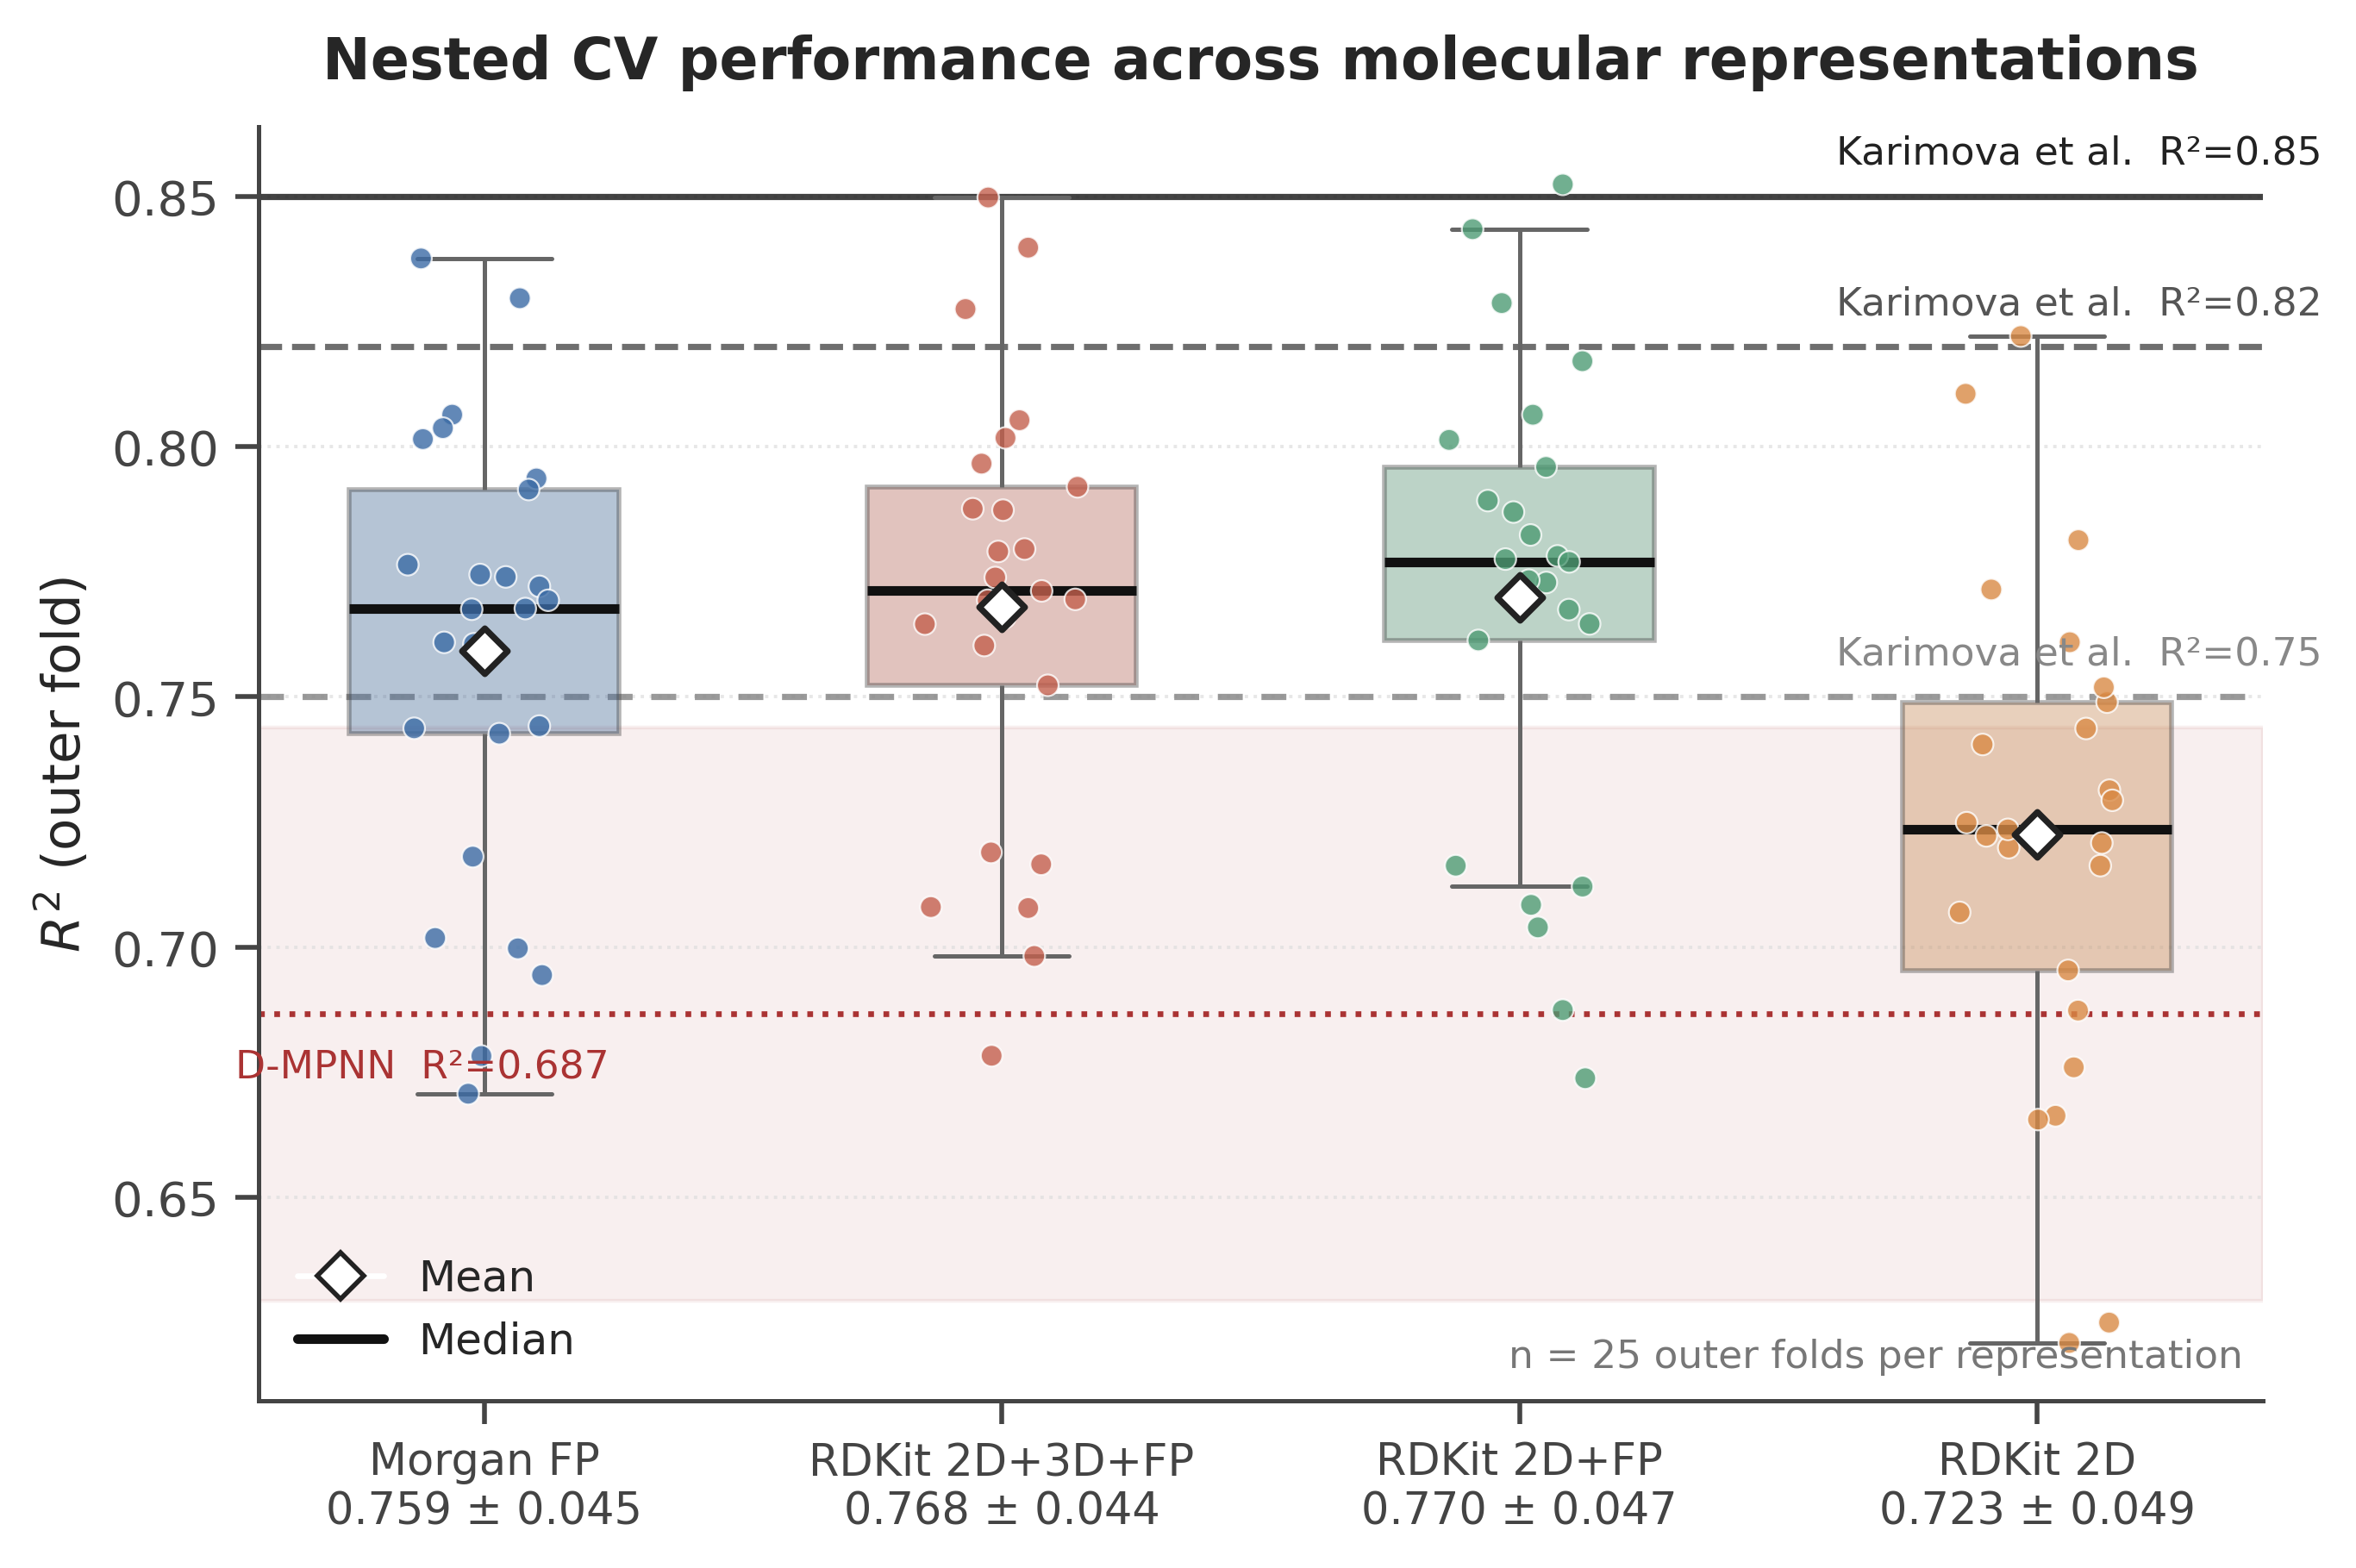
\includegraphics[width=0.8\textwidth]{figures/01_nested_cv_stability_boxplot.png}
	\caption{Nested cross-validation $R^2$ across four molecular representations (each point is one of the 25 outer folds). Horizontal lines mark the three values reported in the original study \cite{karimova2025}; the dotted line and band show the mean $\pm$ SD of the D-MPNN benchmarked in Section~\ref{sec:gnn_results}. The three representations that contain fingerprints are statistically indistinguishable in $R^2$.}
	\label{fig:nested_cv_boxplot}
\end{figure}

Differences between representations were assessed with Nadeau-Bengio corrected paired $t$-tests on the shared outer folds. The three fingerprint-containing spaces could not be separated in $R^2$ (Morgan versus 2D descriptors with fingerprints, $p = \NBpRTwoMorganVsTwoDFp$; Morgan versus the 3D hybrid, $p = \NBpRTwoMorganVsTwoDThreeDFp$; 2D descriptors with fingerprints versus the 3D hybrid, $p = \NBpRTwoTwoDFpVsTwoDThreeDFp$). In MAE, Morgan trailed the two hybrid spaces by \NBdiffMAEMorganVsTwoDFp\ and \NBdiffMAEMorganVsTwoDThreeDFp\ $pIC_{50}$ units ($p = \NBpMAEMorganVsTwoDFp$ and $p = \NBpMAEMorganVsTwoDThreeDFp$), a small gap that is no longer significant after Holm adjustment for the six comparisons ($p_{\mathrm{Holm}} = \NBpHolmMAEMorganVsTwoDFp$ for both). In contrast, 2D descriptors alone were significantly worse than every space that includes fingerprints (versus 2D descriptors with fingerprints, $p = \NBpRTwoTwoDVsTwoDFp$; versus the 3D hybrid, $p = \NBpRTwoTwoDVsTwoDThreeDFp$; versus Morgan, $p = \NBpRTwoMorganVsTwoD$). Topological fingerprints are therefore the primary driver of predictive capacity, and the ten 3D shape descriptors derived from ETKDGv3 embedding and MMFF94 minimization added no measurable advantage for this benchmark.

To rule out chance correlation, a \YRandomNPermutations-iteration y-randomization test was applied to the stacking ensemble of the screening model (\YRandomArchitecture: random forest, XGBoost and SVR with a ridge meta-learner) trained on Morgan fingerprints and scored by \YRandomCVFolds-fold cross-validation. With the true potencies this model reached $R^2 = \YRandomTrueRTwo$ (a single \YRandomCVFolds-fold partition, which explains the small difference from the nested estimate), whereas the permuted models collapsed to a mean $R^2$ of $\YRandomMeanRTwo \pm \YRandomStdRTwo$, a separation of $Z = \YRandomZScore$ standard deviations. The ensemble therefore maps genuine structure--activity relationships rather than memorizing noise.

Selection of the stacking architecture was unstable (Figure~\ref{fig:algorithm_selection}). Within the Morgan space, Support Vector Regression entered the selected ensemble in \SelMorganSVMPct\% of the outer folds and Random Forest in \SelMorganRFPct\%, followed by XGBoost (\SelMorganXGBPct\%), LightGBM (\SelMorganLGBMPct\%), $k$-nearest neighbors (\SelMorgankNNPct\%), and Extra Trees (\SelMorganETPct\%); the selected ensembles contained one, two, or three models in \SelMorganSizeOnePct\%, \SelMorganSizeTwoPct\%, and \SelMorganSizeThreePct\% of the folds. No single hierarchy dominated: the most frequent exact combination, \MorganBestArchitecture, won only \MorganStability\% of the folds (\SelMorganTopCount/\TotalOuterFolds), followed by \SelMorganSecond\ (\SelMorganSecondCount/\TotalOuterFolds) and \SelMorganNOthers\ further architectures selected in at most \SelMorganOthersMaxCount\ folds each. The descriptor-based spaces behaved differently: Extra Trees was selected in \SelRdkitTwoDETPct\%, \SelRdkitTwoDFpETPct\%, and \SelRdkitTwoDThreeDFpETPct\% of the folds of the 2D, 2D+FP, and 2D+3D+FP spaces, respectively, and SVR in \SelRdkitTwoDSVMPct\%, \SelRdkitTwoDFpSVMPct\%, and \SelRdkitTwoDThreeDFpSVMPct\%. While aggregated performance remains stable across outer folds, the data sparsity of the \NCompounds-compound benchmark prevents the inner loop from isolating a universally superior ensemble.

\begin{figure}[htbp]
	\centering
	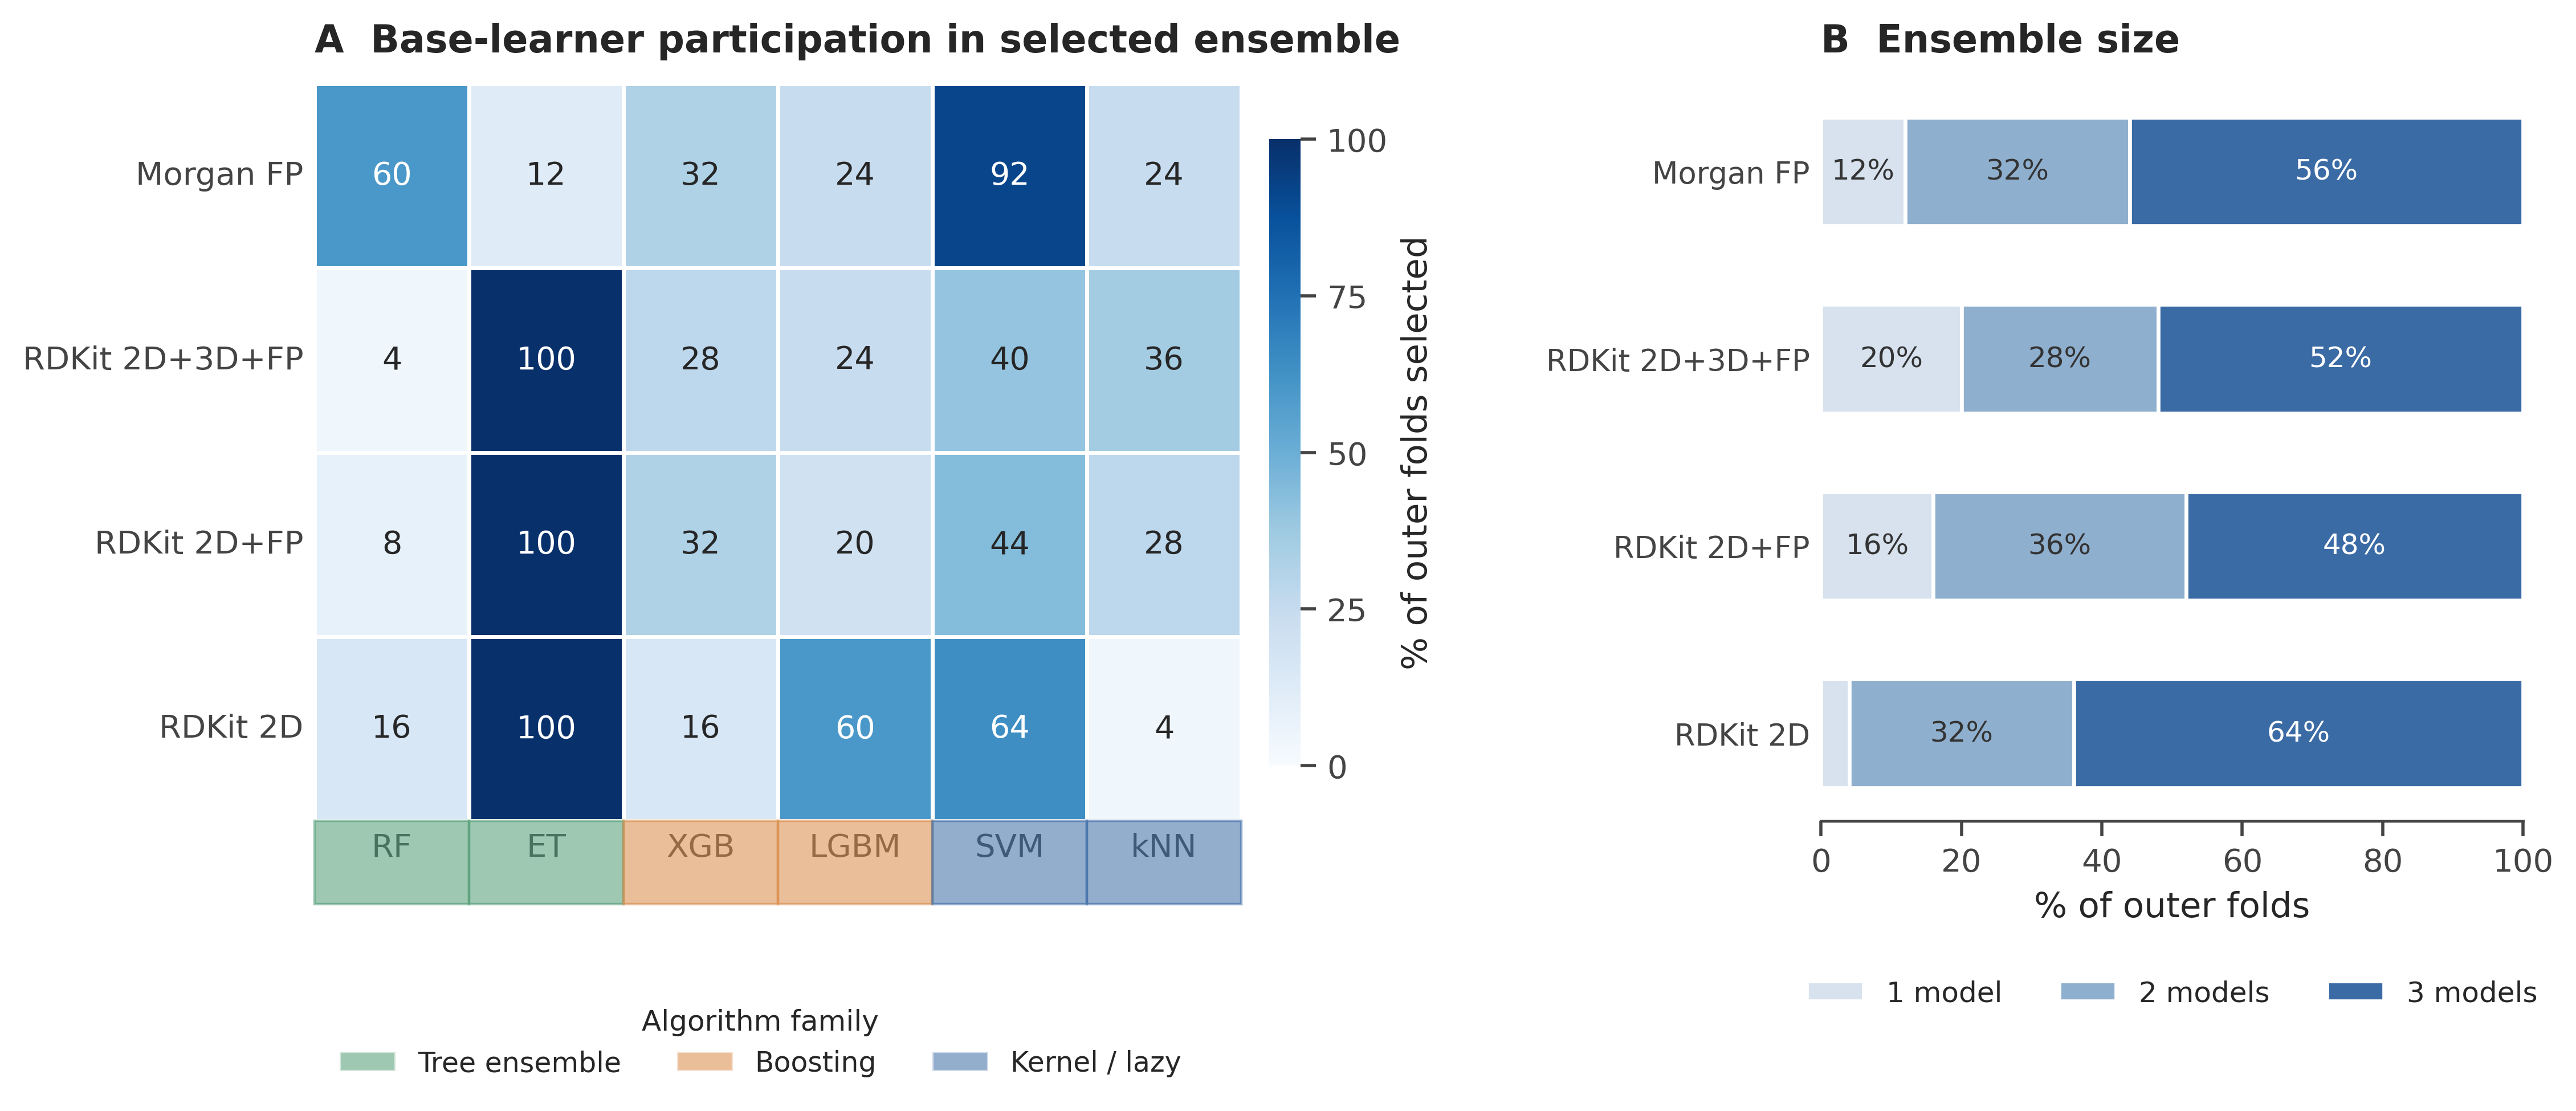
\includegraphics[width=\textwidth]{figures/01_nested_cv_algorithm_selection.png}
	\caption{Composition of the stacking ensembles selected by the inner loop in the 25 outer folds. (A) Percentage of folds in which each base learner entered the selected ensemble, per representation. (B) Distribution of ensemble size (one, two, or three base models). No single architecture dominates in the Morgan space.}
	\label{fig:algorithm_selection}
\end{figure}

We then placed these results against the incremental progression reported in the original study (Table~\ref{tab:methodological_comparison}). Our classical stacking ensemble trained solely on Morgan features ($R^2 = \MorganRTwoMean$) performed comparably to their unselected 2D/3D/FP baseline ($R^2 = \PaperBaselineRTwo$); under a Nadeau-Bengio corrected one-sample $t$-test the difference was not significant ($t = \TStatMorganVsPaperBaseline$, $p = \PValueMorganVsPaperBaseline$). In contrast, the literature value for the model with permutation-importance feature selection ($R^2 = \PaperSelectedRTwo$) lies significantly above our nested cross-validated Morgan estimate ($t = \TStatMorganVsPaperSelected$, $p = \PValueMorganVsPaperSelected$), and so does the final data-augmented deep neural network ensemble ($R^2 = \PaperFinalRTwo$; $t = \TStatMorganVsPaperFinal$, $p = \PValueMorganVsPaperFinal$). This comparison has a limitation: the original values come from a single hold-out split without a reported dispersion and are treated here as fixed constants, so the test does not capture the sampling variability of that split. Achieving a competitive baseline ($R^2 \approx \PaperBaselineRTwo$) does not require computationally expensive 3D descriptors or complex neural network architectures; simple 2D fingerprints paired with classical algorithms suffice.

\begin{table}[htbp]
	\centering
	\caption{Methodological comparison isolating the performance impact of architectural complexity, descriptor dimensionality, and data augmentation in TgDHFR bioactivity prediction.}
	\label{tab:methodological_comparison}
	\small
	\begin{tabular}{@{}>{\raggedright\arraybackslash}p{0.35\textwidth}p{0.2\textwidth}p{0.13\textwidth}p{0.2\textwidth}@{}}
		\toprule
		\textbf{Model Framework} & \textbf{Descriptors} & \shortstack[l]{\textbf{Data}\\\textbf{Augmentation}} & \shortstack[l]{\textbf{Test $R^2$}\\\textbf{(mean $\pm$ std)}} \\
		\midrule
		Current Study (Classical Ensemble) & ECFP4 (2D) & None & \MorganRTwoMean $\pm$ \MorganRTwoStd \\
		Baseline \cite{karimova2025} & 2D/3D/FP & None & \PaperBaselineRTwo \textsuperscript{a} \\
		Feature-selected model \cite{karimova2025} & 2D/3D/FP (Selected) & None & \PaperSelectedRTwo \textsuperscript{a} \\
		Augmented Final Model \cite{karimova2025} & 2D/3D/FP (Selected) & Gaussian Noise & \PaperFinalRTwo \textsuperscript{a} \\
		\bottomrule
		\multicolumn{4}{p{0.9\textwidth}}{\footnotesize \textsuperscript{a} Standard deviation not reported (NR) in the original study.}
	\end{tabular}
\end{table}

To test whether the interventions credited with the gains of the original study transfer to classical learners, we replicated its protocol (15\% hold-out, seed 42; \ExpNTest\ molecules held out before any selection or augmentation, \ExpNDev\ for development) on a stacking ensemble (Figure~\ref{fig:augmentation_ablation}). The unselected baseline reached $R^2 = \ExpARTwoMean$ (MAE = \ExpAMae). Permutation-importance selection (\ExpBNFeaturesSelected\ of \ExpBNFeaturesTotal\ bits retained) yielded $R^2 = \ExpBRTwoMean$ (MAE = \ExpBMae), and Gaussian-noise augmentation yielded $R^2 = \ExpCRTwoMean$ (MAE = \ExpCMae). Paired bootstrap differences showed no significant effect of either intervention: selection changed $R^2$ by $\ExpBvsADeltaRTwo$ (95\% CI $[\ExpBvsADeltaCILow, \ExpBvsADeltaCIHigh]$) and augmentation by $\ExpCvsADeltaRTwo$ (95\% CI $[\ExpCvsADeltaCILow, \ExpCvsADeltaCIHigh]$) relative to the baseline, and both intervals include zero. The hold-out intervals are wide, spanning roughly 0.2 $R^2$ units, and contain the original baseline of \PaperBaselineRTwo; the original values of \PaperSelectedRTwo\ and \PaperFinalRTwo\ lie above the upper limits of the intervals for selection ($p_{\mathrm{boot}} = \ExpBVsPaperSelectedPBoot$) and augmentation ($p_{\mathrm{boot}} = \ExpCVsPaperFinalPBoot$), respectively. The gains reported for the original deep ensemble were therefore not reproduced by feature selection or augmentation applied to a classical learner; they may depend on the neural architecture, or reflect the sampling variability of a single hold-out split. Two properties of the replicated interventions limit how strong this negative result is. First, the permutation importance was computed on the data the model was fitted on, so the selection removes essentially the bits the model never uses and little else, and no change is expected for tree-based learners. Second, Gaussian noise of $\sigma \leq 0.01$ added to binary fingerprint bits barely moves the split thresholds of tree models, so the augmented copies are almost identical to the originals. Neither intervention was therefore a demanding test of its idea.

\begin{figure}[htbp]
	\centering
	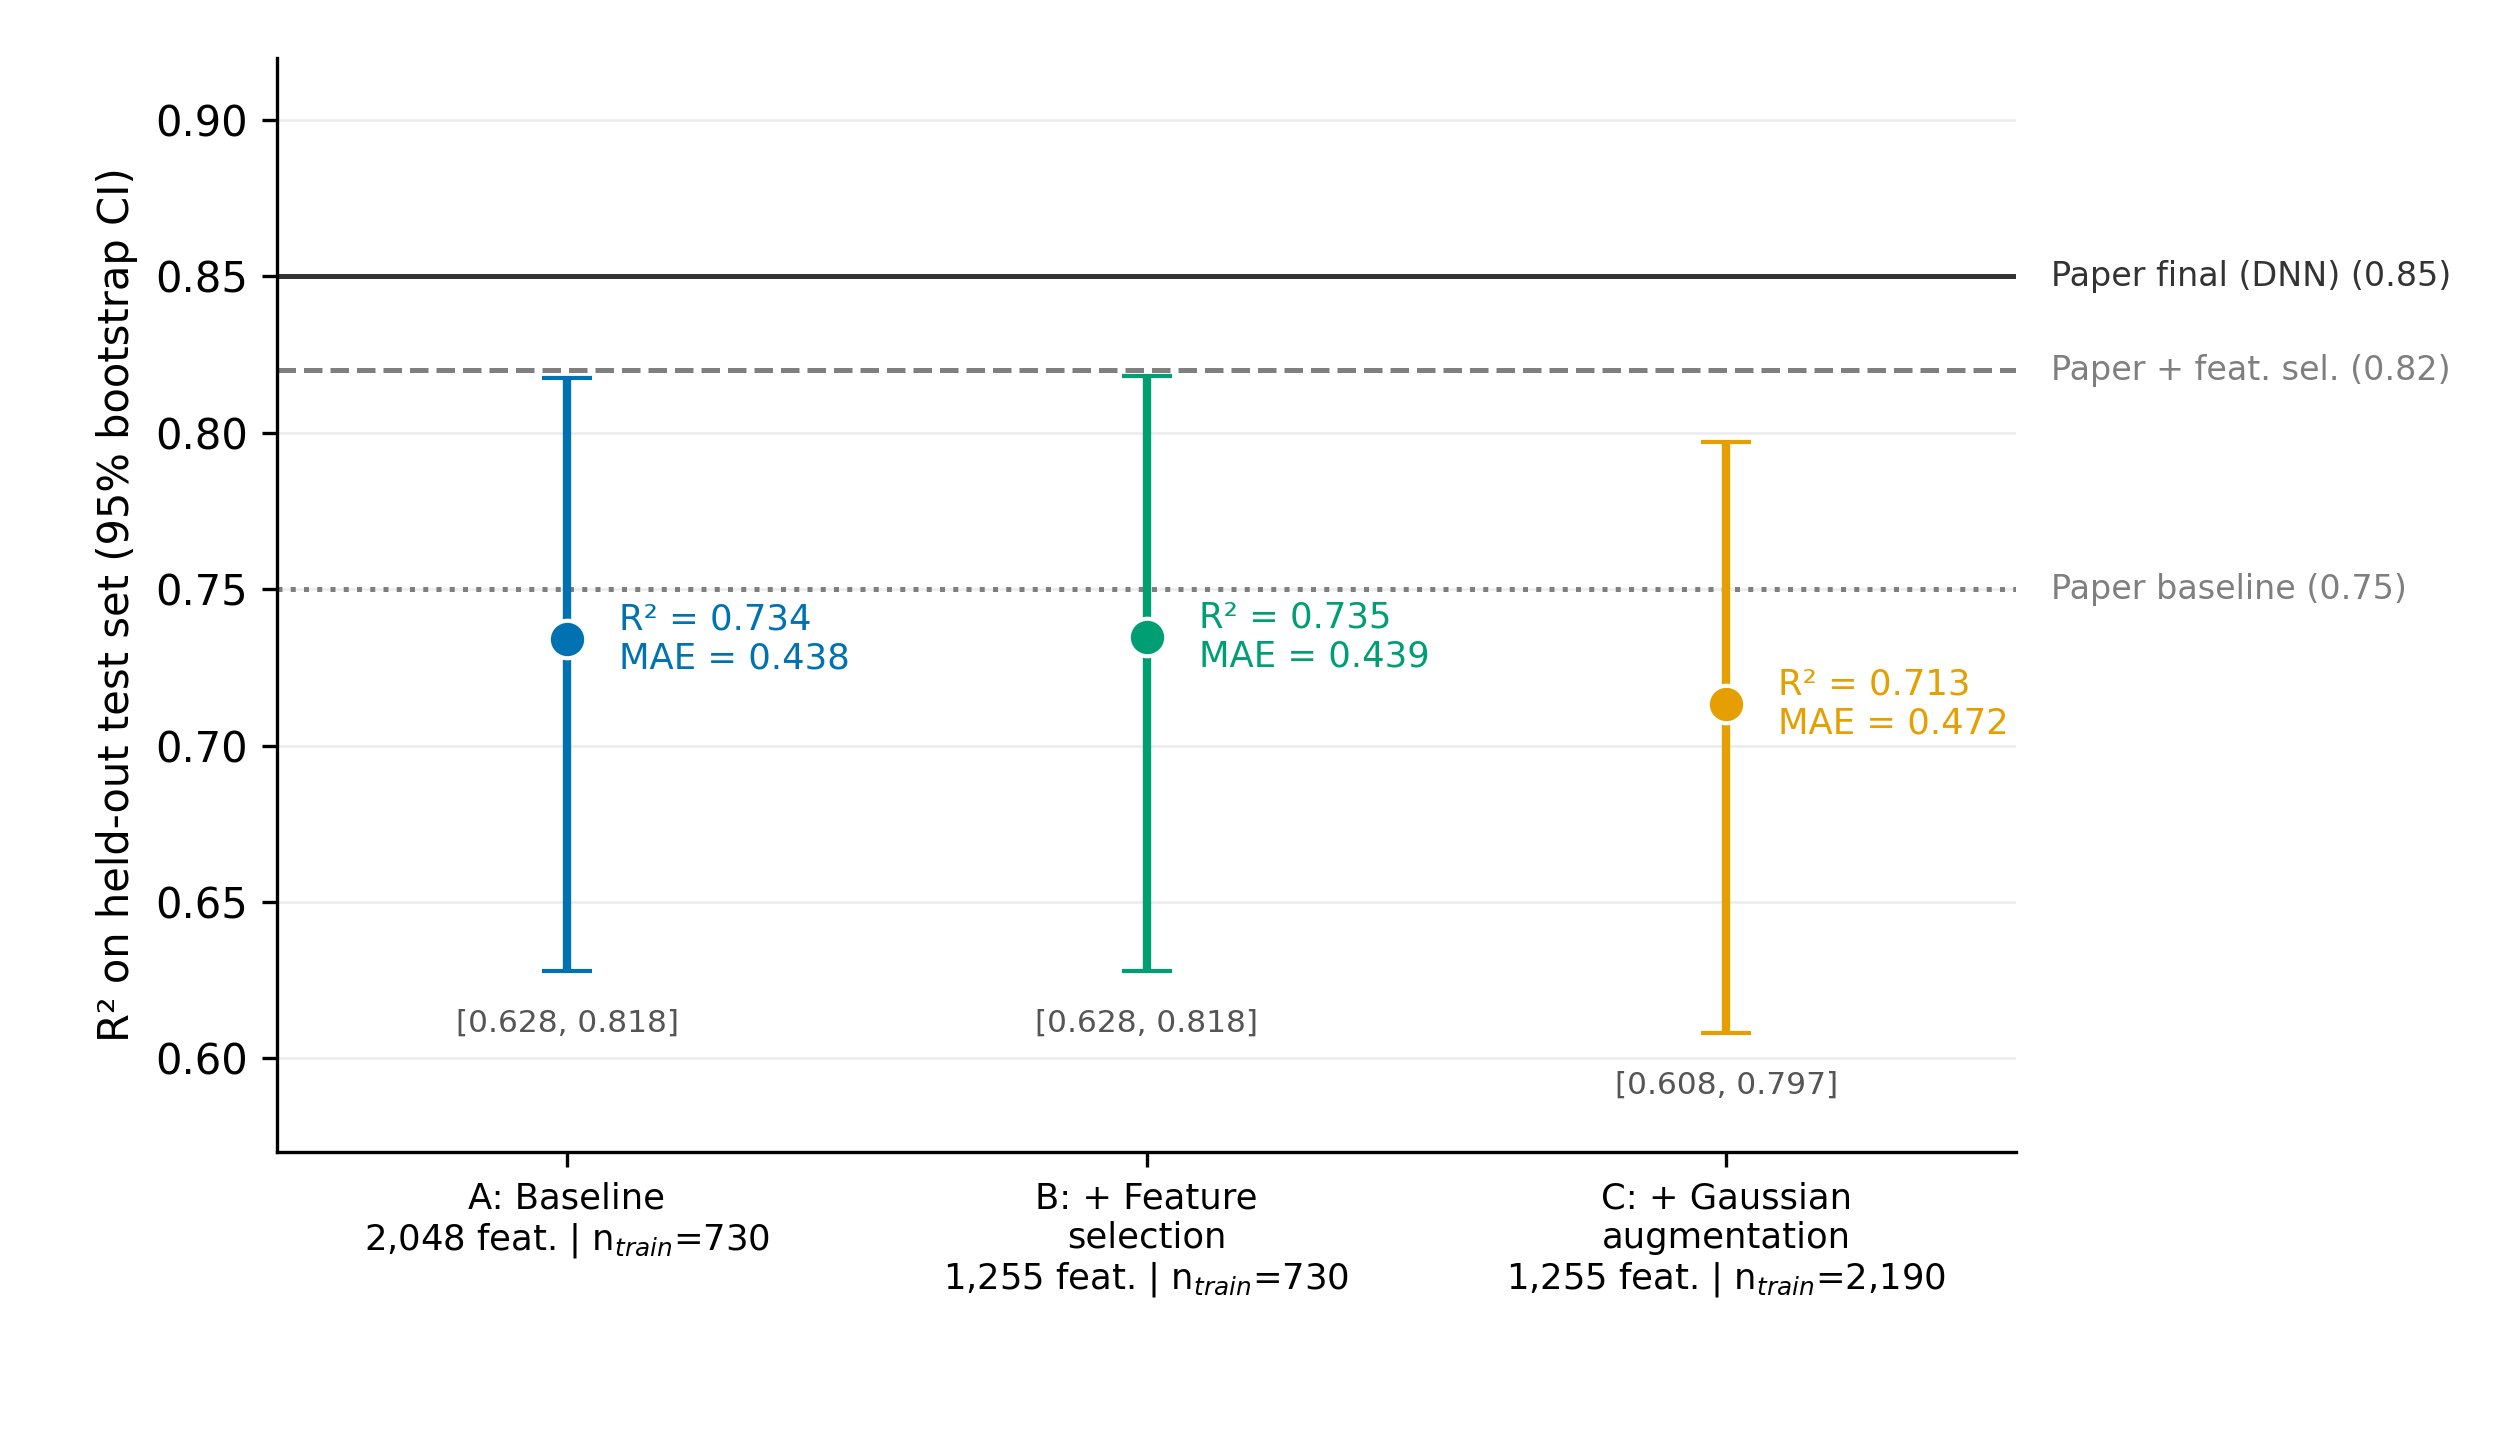
\includegraphics[width=0.8\textwidth]{figures/04_augment_r2_comparison.png}
	\caption{Replication of the original hold-out protocol on a classical stacking ensemble (\ExpNTest\ held-out molecules). Points are $R^2$ on the test set with 95\% bootstrap confidence intervals for the baseline (A), permutation-importance feature selection (B), and feature selection plus Gaussian-noise augmentation (C); horizontal lines mark the values reported in the original study \cite{karimova2025}.}
	\label{fig:augmentation_ablation}
\end{figure}

% ==========================================
% 3. SECTION 3.2
% ==========================================
\subsection{Benchmarking Tree-Based Ensembles Against Graph Neural Networks}
\label{sec:gnn_results}

Graph neural networks learn molecular representations directly from the atom--bond graph, but their advantage is expected to shrink when labeled data are scarce. To test whether representation learning helps on the TgDHFR dataset (\NCompounds\ compounds), a Directed Message Passing Neural Network (D-MPNN, Chemprop) was evaluated on exactly the same \TotalOuterFolds\ outer folds as the classical ensembles, in two variants described in the Methods: default hyperparameters, and a hyperparameter search nested inside each outer fold.

The default D-MPNN reached a mean fold $R^2$ of $\ChemPropDMPNNFoldRTwoMean \pm \ChemPropDMPNNFoldRTwoStd$ and a mean absolute error of \ChemPropDMPNNFoldMae, compared with $R^2 = \MorganRTwoMean \pm \MorganRTwoStd$ for the Morgan-fingerprint stacking ensemble (Figure~\ref{fig:gnn_comparison}). Because the folds are shared, the models can be compared with the same Nadeau--Bengio corrected paired $t$-test used for the classical representations. The network was numerically below the Morgan ensemble ($\Delta R^2 = \GnnVsMorganDiffRTwo$) and the fingerprint-based hybrid ensembles ($\Delta R^2 = \GnnVsRdkitTwoDFpDiffRTwo$ and $\GnnVsRdkitTwoDThreeDFpDiffRTwo$ against 2D+FP and 2D+3D+FP), and on par with the 2D descriptors alone ($\Delta R^2 = \GnnVsRdkitTwoDDiffRTwo$), but no difference was significant after Holm adjustment (smallest adjusted $p$: \GnnVsMinPRTwo\ for $R^2$ and \GnnVsMinPMae\ for MAE).

Tuning did not change this picture. In the nested search, the selected configuration varied across folds (\GnnTunedNChosen\ of the \GnnTunedNConfigs\ configurations were chosen at least once, and the default one in only \GnnTunedDefaultChosenPct\% of the folds), but the tuned network reached $R^2 = \GnnTunedRTwoMean \pm \GnnTunedRTwoStd$ and MAE = \GnnTunedMae, indistinguishable from the default one ($\Delta R^2 = \GnnTunedVsUntunedDiffRTwo$, $p = \GnnTunedVsUntunedPRTwo$; $\Delta$MAE $= \GnnTunedVsUntunedDiffMae$, $p = \GnnTunedVsUntunedPMae$). Against the classical ensembles the tuned network was again numerically lower than Morgan ($\Delta R^2 = \GnnTunedVsMorganDiffRTwo$, Holm-adjusted $p = \GnnTunedVsMorganPRTwo$) and the two fingerprint-based hybrids ($\Delta R^2 = \GnnTunedVsRdkitTwoDFpDiffRTwo$ and $\GnnTunedVsRdkitTwoDThreeDFpDiffRTwo$), and on par with the 2D descriptors ($\Delta R^2 = \GnnTunedVsRdkitTwoDDiffRTwo$); none of these differences was significant (smallest adjusted $p$: \GnnTunedVsMinPRTwo\ for $R^2$ and \GnnTunedVsMinPMae\ for MAE).

Equivalence is a separate question. With the $\pm 0.05$ margin, the tuned network was equivalent to the 2D descriptors in $R^2$ (90\% CI $[\GnnTunedVsRdkitTwoDCILowRTwo, \GnnTunedVsRdkitTwoDCIHighRTwo]$, $p = \GnnTunedVsRdkitTwoDEquivPRTwo$), but equivalence to the Morgan ensemble could not be shown for $R^2$ (90\% CI $[\GnnTunedVsMorganCILowRTwo, \GnnTunedVsMorganCIHighRTwo]$, $p = \GnnTunedVsMorganEquivPRTwo$). In MAE, the tuned network and the Morgan ensemble were equivalent within $\pm 0.05$ ($\Delta = \GnnTunedVsMorganDiffMae$, 90\% CI $[\GnnTunedVsMorganCILowMae, \GnnTunedVsMorganCIHighMae]$, $p = \GnnTunedVsMorganEquivPMae$). The evidence therefore supports that the network is not clearly worse in absolute error, but leaves open a deficit in $R^2$ as large as $\Delta R^2 = \GnnTunedVsMorganCILowRTwo$. The tuned search was deliberately modest (Methods), so a larger search or a different architecture could change this.

Both graph-network variants and the classical ensembles fall in the same range as the original study's unselected baseline ($R^2 = \PaperBaselineRTwo$). The final augmented ensemble of the original study ($R^2 = \PaperFinalRTwo$) lies above this range, but, as discussed in Section~\ref{sec:res_classical}, that value comes from a single hold-out split and was not reproduced by selection or augmentation on a classical learner. Under the data volume of this benchmark, the graph architecture therefore did not provide a measurable gain over fixed fingerprints.

Computational cost does not favor the classical approach in this protocol, but the comparison needs care (Table~\ref{tab:cost}). One default D-MPNN training took about \GnnFoldSecMean\ s on the workstation CPU (about \GnnTotalMin\ minutes for the \TotalOuterFolds\ folds), whereas a classical outer fold with its complete inner search took between \ClassicalFoldSecMin\ and \ClassicalFoldSecMax\ s depending on the representation (\ClassicalMorganFoldSec\ s, about \ClassicalMorganTotalHours\ h in total, for Morgan). The default network received no model selection. When it did, in the tuned variant, one outer fold took \GnnTunedFoldSecMean\ s, about \GnnTunedTotalHours\ h of worker time for the whole benchmark, which is more than the classical protocol even though the network's search was smaller. The case for the classical ensembles therefore rests on accuracy that is not lower, on simpler inputs and models that run on a CPU, and on a deployed model that uses only a subset of the fingerprint bits, and not on a shorter benchmark.

\begin{table}[htbp]
	\centering
	\caption{Run time and accuracy of every model. Time is the mean wall-clock time of one outer fold on the workstation, including the inner search where one exists, and the 25-fold total is that time multiplied by 25. Times are not normalized by thread count (the classical models used all threads on one fold at a time; the tuned D-MPNN ran two training processes in parallel).}
	\label{tab:cost}
	\resizebox{\textwidth}{!}{% Auto-generated by 09.1_build_figures.py
\begin{tabular}{lcccc}
\toprule
\textbf{Model} & \textbf{Time per outer fold (s)} & \textbf{25 folds (h)} & \textbf{Model selection} & $R^2$ \\
\midrule
Morgan FP & 1987 & 13.8 & Yes (41 combinations) & $0.769 \pm 0.041$ \\
RDKit 2D+FP & 2504 & 17.4 & Yes (41 combinations) & $0.774 \pm 0.043$ \\
RDKit 2D+3D+FP & 2586 & 18.0 & Yes (41 combinations) & $0.774 \pm 0.041$ \\
RDKit 2D & 1182 & 8.2 & Yes (41 combinations) & $0.728 \pm 0.048$ \\
D-MPNN, default & 179 & 1.2 & No & $0.725 \pm 0.043$ \\
D-MPNN, tuned & 2192 & 15.2 & Yes (8 configurations) & $0.726 \pm 0.034$ \\
\bottomrule
\end{tabular}
}
\end{table}

\begin{figure}[htbp]
	\centering
	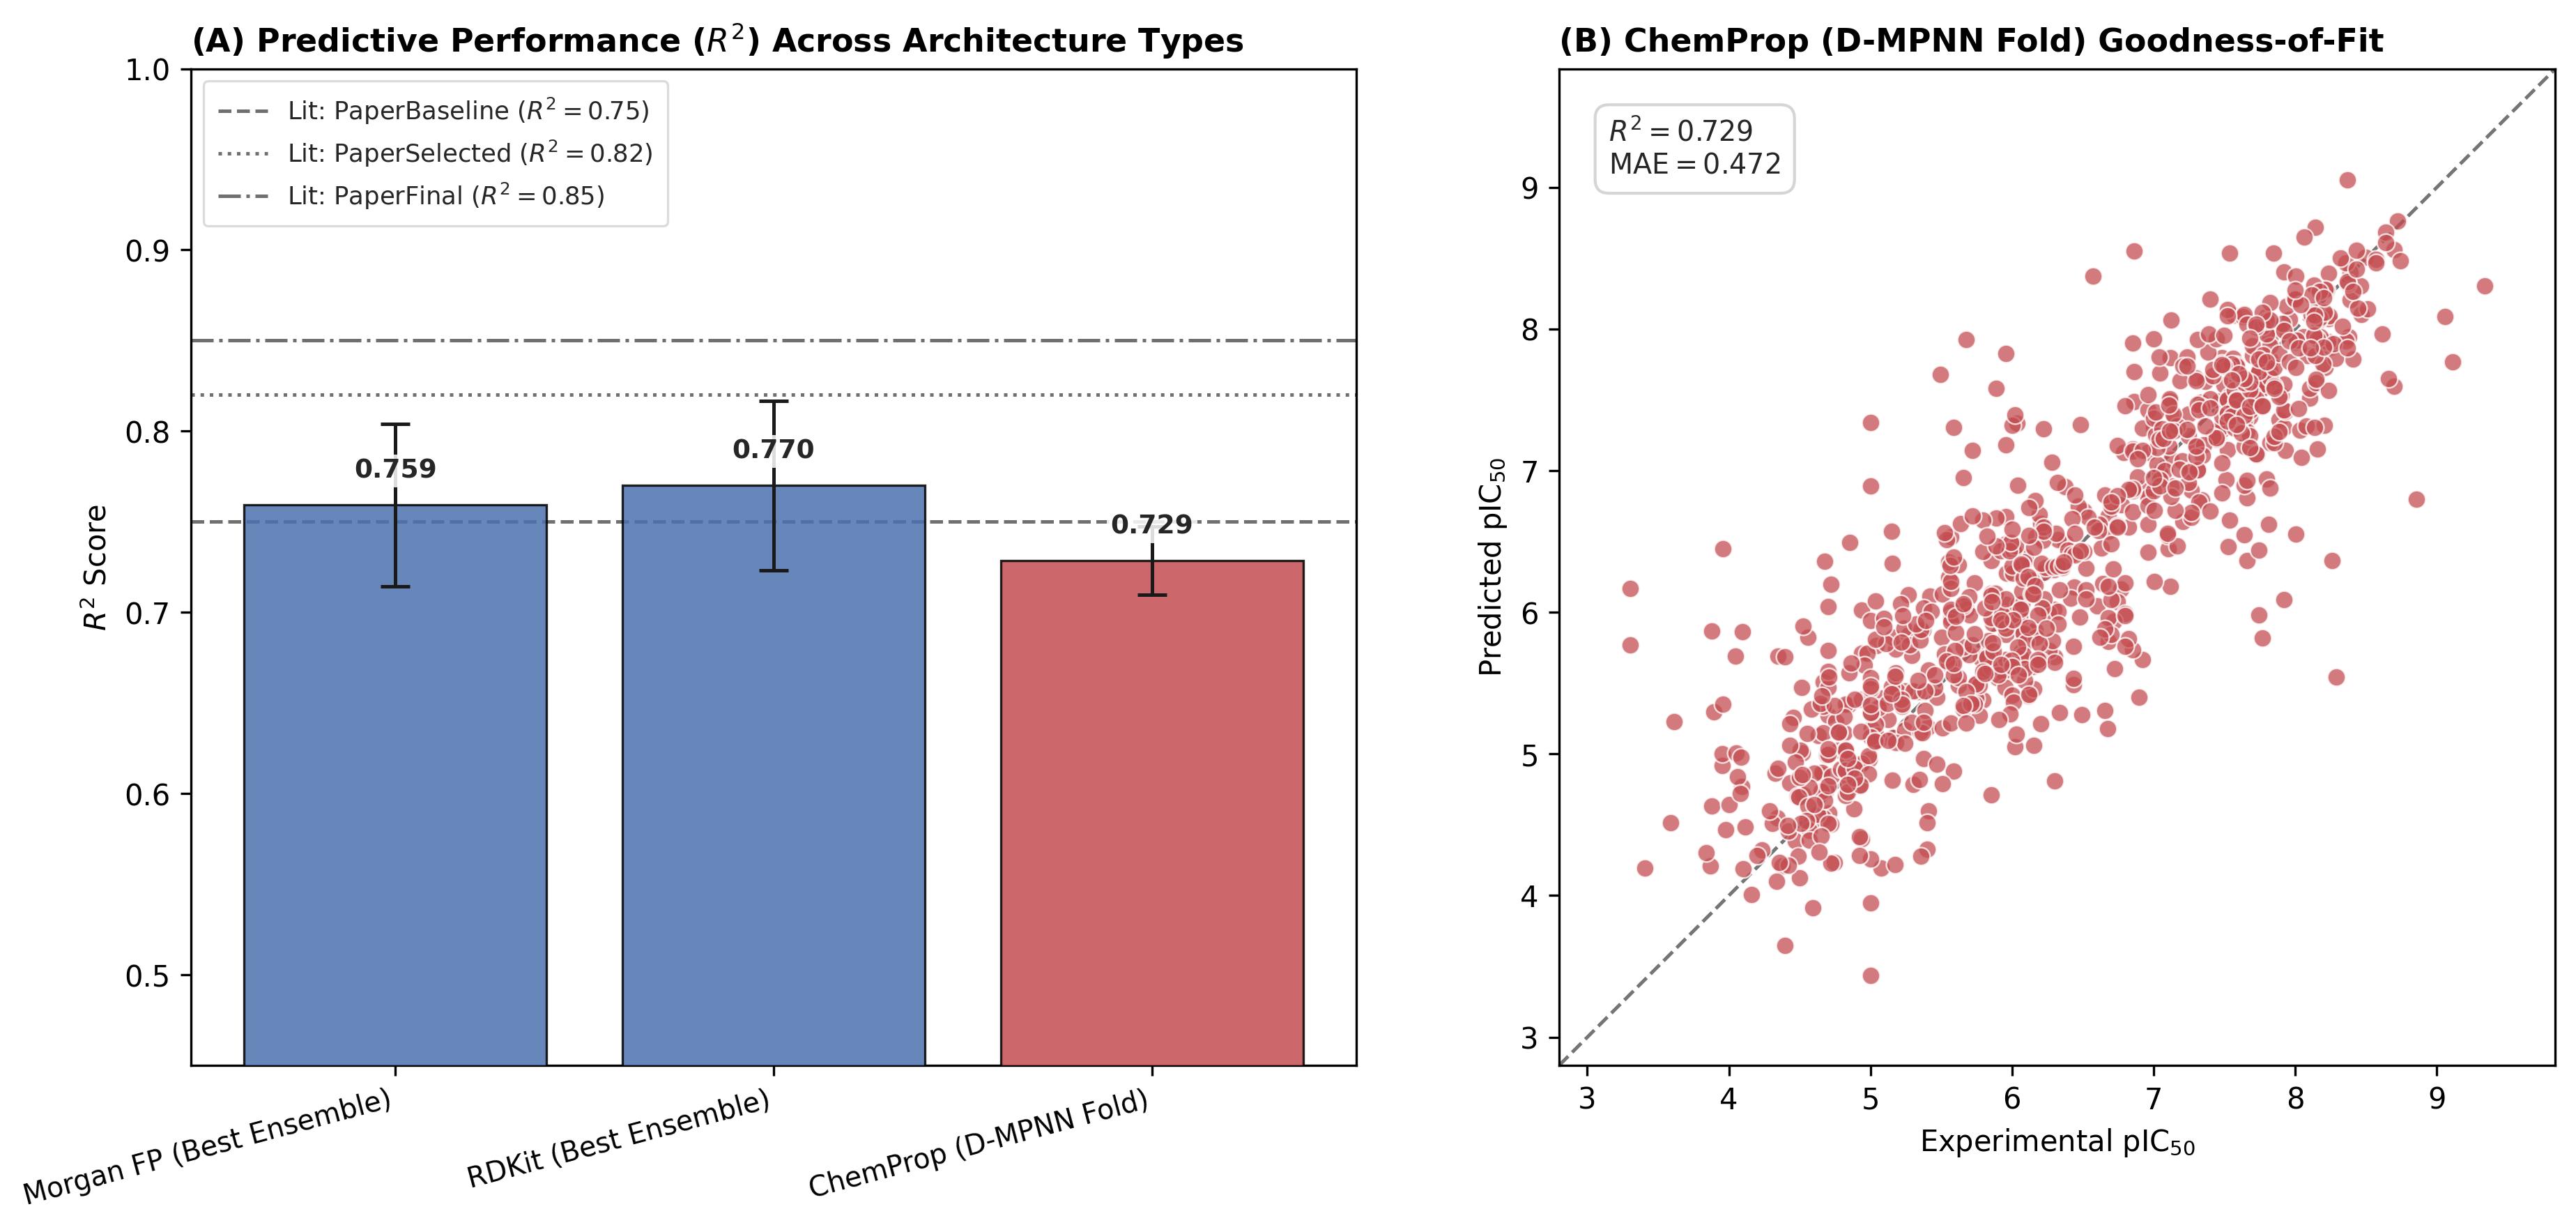
\includegraphics[width=\textwidth]{figures/09_gnn_benchmark_comparison.png}
	\caption{(A) Mean $R^2$ over the \TotalOuterFolds\ shared outer folds for the best classical ensembles and the D-MPNN with default and tuned hyperparameters; error bars are the standard deviation across folds, and horizontal lines mark the values reported in the original study. (B) Default D-MPNN predicted versus experimental pIC$_{50}$ for every compound, averaged over the five repeats of the cross-validation (each prediction comes from a model that did not see the compound).}
	\label{fig:gnn_comparison}
\end{figure}

% ==========================================
% 3. SECTION 3.3 (screening, docking and ADMET: hypothesis generation)
% ==========================================
\subsection{Hypothesis Generation: Screening, Docking and ADMET}
\label{sec:screening_results}
\label{sec:consensus_results}
\label{sec:admet_results}

The deployed model, the feature-selected Morgan-fingerprint stacking ensemble of the augmentation experiment (Section~\ref{sec:res_classical}), was applied to the FDA-approved library after the funnel described in the Methods: \ScreenNLibrary{} compounds were reduced to \ScreenNStructural{} by the size and elemental filters, and all of these were scored. Their mean Tanimoto similarity to the five most similar training compounds had a median of \ScreenADFdaMedian{} (5th--95th percentile \ScreenADFdaLow{}--\ScreenADFdaHigh{}), against \ScreenADTrainMedian{} for the training compounds measured against each other, and only \ScreenNDomain{} of them reached the applicability-domain threshold of \ScreenADMinSimilarity{}. The predicted potencies of this library are therefore mostly extrapolations, and each candidate's similarity to the training set is reported with its prediction; of the \ScreenNCandidates{} candidates advanced to docking, \ScreenNCandidatesInDomain{} were inside the domain. As a consistency check, pyrimethamine was predicted at pIC$_{50}$ \ControlPyrimethaminePred{} (experimental \ControlPyrimethamineExp{}) and trimethoprim at \ControlTrimethoprimPred{} (experimental \ControlTrimethoprimExp{}); both belong to the training partition, so this verifies that the final model fits its training data and says nothing about generalization.

Table~S1 and Figures~S3--S5 give the ranking with its efficiency metrics. The antifolates methotrexate, trimetrexate and pralatrexate lead by absolute potency, but potency scales with molecular size and their efficiency is modest (ligand efficiency between \AntifolateLEMin{} and \AntifolateLEMax{}, against the value of 0.30 commonly taken as the lower bound of a good lead); methotrexate is also in the training set, so its rank partly reflects memorization. Size-corrected metrics reorder the list: triamterene, which is absent from the training data, combines a predicted pIC$_{50}$ of \CandTriamterenePred{} with the highest ligand efficiency (\CandTriamtereneLE{}) and binding efficiency index (\CandTriamtereneBEI{}) of the table, and is therefore the clearest repurposing hypothesis of the ML stage.

Because neither ligand-based prediction nor docking is reliable alone, the \DockNTotal{} candidates were scored by both and classified by agreement (Figure~\ref{fig:docking_scatter}), a compound being a consensus hit when the model predicts it active ($pIC_{50} > \DockMLActiveThresh$) and it docks favorably ($\Delta G < \DockActiveThresh\text{ kcal/mol}$). This yielded \DockNValidated{} entries (\DockNValidatedUnique{} unique compounds): pralatrexate ($pIC_{50} = \PralatrexateMLpIC$, $\Delta G = \PralatrexateDockScore$ kcal/mol, the best docking score of the set), methotrexate (\MethotrexateMLpIC, \MethotrexateDockScore), trimetrexate glucuronate (\TrimetrexateMLpIC, \TrimetrexateDockScore) and triamterene (\TriamtereneMLpIC, \TriamtereneDockScore). Agreement between the two methods is weak: Spearman's rank correlation between predicted $pIC_{50}$ and Vina score was $\rho = \DockSpearmanRho$ ($p = \DockSpearmanP$), with the expected sign but no statistical significance, and the estimate is less informative than its $N = \DockNTotal$ suggests, because the four trimethoprim entries share one structure and one docking score. We therefore read the correlation only as evidence that docking does not reproduce the ML ranking.

The discordant cases bound both methods. Pyrimethamine, an established TgDHFR inhibitor, docked at only $\Delta G = \PyrimethamineDockScore$ kcal/mol and trimethoprim similarly ($\Delta G = \TrimethoprimDockScore$ kcal/mol); small ligands obtain modest Vina scores because the score grows with the number of contacts, which points to a limited sensitivity of the scoring function for small inhibitors rather than to an ML artifact. Bisacodyl is the opposite case, favored by docking ($\Delta G = \BisacodylDockScore$ kcal/mol) while the model predicted $pIC_{50} = \BisacodylMLpIC$; it carries none of the diaminopyrimidine-like features of the antifolate ligands in the training set, so a docking artifact of a flexible, hydrophobic ligand is the more plausible explanation. Without experimental data we cannot arbitrate between the two methods.

\begin{figure}[htbp]
	\centering
	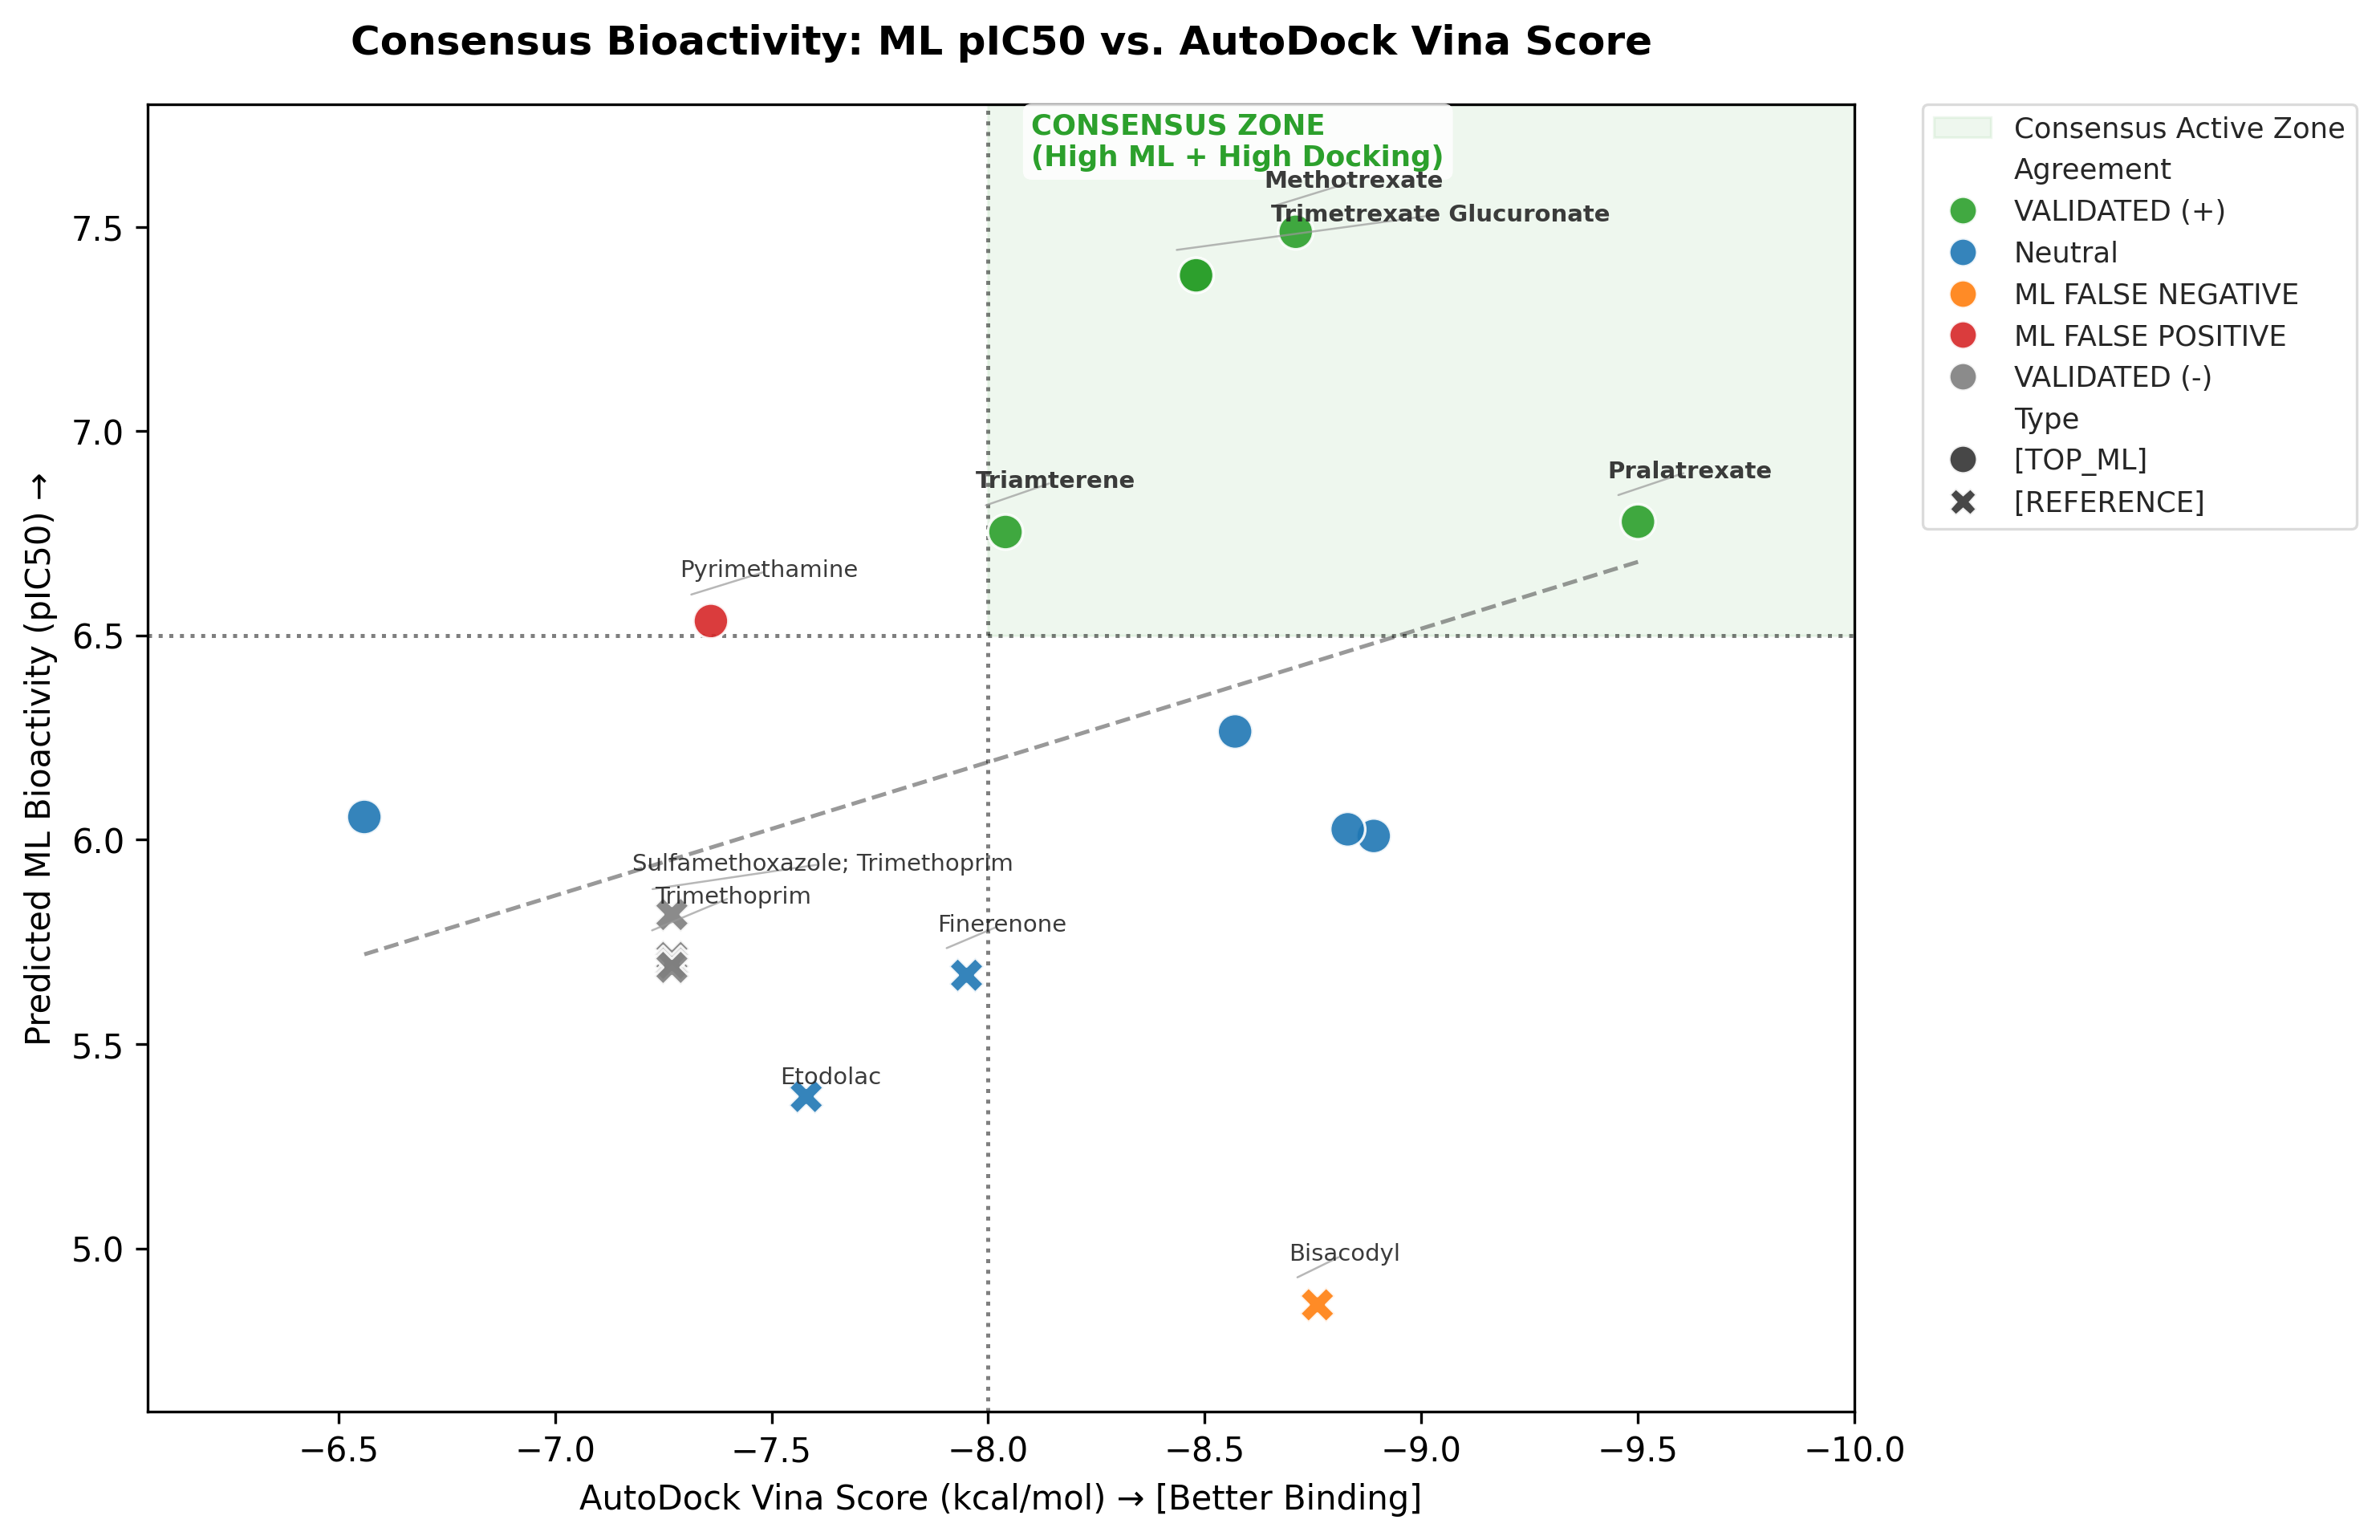
\includegraphics[width=0.9\textwidth]{figures/07_docking_scatter.png}
	\caption{Predicted pIC$_{50}$ versus AutoDock Vina score for the \DockNTotal{} docked candidates, coloured by agreement class. The shaded region is the consensus zone ($pIC_{50} > \DockMLActiveThresh$ and $\Delta G < \DockActiveThresh$ kcal/mol).}
	\label{fig:docking_scatter}
\end{figure}

Of the \AdmetNDocked{} docked entries, \AdmetNLipinski{} satisfied the three Lipinski criteria, the hERG classifier flagged \AdmetNHergFlagged{} as likely channel blockers, and \AdmetNRemaining{} remained: \AdmetNOral{} classified as oral and \AdmetNParenteral{} as parenteral because of low predicted Caco-2 permeability (Table~S2, Figure~S6). Of the \AdmetNConsensus{} consensus hits, \AdmetNConsensusSurvivors{} passed both filters: pralatrexate and methotrexate were hERG-safe but poorly permeable and so classified as parenteral, and trimetrexate was predicted to be hERG-safe and orally absorbed, whereas triamterene, the most ligand-efficient candidate of the screen, was the only consensus hit removed (predicted hERG probability \AdmetHergTriamterene{}). How much weight such a profile deserves depends on the indication and the length of the course: toxoplasmosis is treated for weeks, far longer in ocular and immunocompromised cases, and its cerebral and congenital forms require passage of the blood--brain barrier and the placenta, so the filter is informative for this target, but it is a rule- and classifier-based screen and not part of the benchmark.

This whole stage is a computational prioritization. The receptor is rigid, no water molecules or protonation states are modelled, Vina scores are empirical estimates, and the ADMET classifiers were trained on public data whose accuracy was not evaluated here, with some of these compounds in their training sets. The consensus hits are therefore hypotheses for experimental testing and not confirmed inhibitors.

% ==========================================
% 3. SECTION 3.6
% ==========================================
\subsection{Robustness to Scaffold-Grouped Splits}
\label{sec:scaffold_results}

Random folds place close analogs of a test compound in the training set, which favors models that memorize local structure. To measure how much of the reported accuracy depends on this, the Morgan-fingerprint ensemble and the D-MPNN were re-evaluated with scaffold-grouped outer folds (Section~\ref{sec:materials_ncv}), keeping the \TotalOuterFolds\ folds, the hyperparameters and the shared partitions. Table~\ref{tab:scaffold} summarizes the outcome.

\begin{table}[htbp]
	\centering
	\caption{Cross-validated performance (mean $\pm$ SD over \TotalOuterFolds\ outer folds) under random and scaffold-grouped splits. The drop is the difference in mean $R^2$.}
	\label{tab:scaffold}
	\begin{tabular}{lcccc}
		\hline
		Model & $R^2$ (random) & $R^2$ (scaffold) & Drop in $R^2$ & MAE (scaffold) \\
		\hline
		Morgan ensemble & $\RandomMorganRTwoMean \pm \RandomMorganRTwoStd$ & $\ScaffoldMorganRTwoMean \pm \ScaffoldMorganRTwoStd$ & \ScaffoldMorganDropRTwo & \ScaffoldMorganMae \\
		D-MPNN & $\RandomGnnRTwoMean \pm \RandomGnnRTwoStd$ & $\ScaffoldGnnRTwoMean \pm \ScaffoldGnnRTwoStd$ & \ScaffoldGnnDropRTwo & \ScaffoldGnnMae \\
		\hline
	\end{tabular}
\end{table}

Both families lost about 0.2 units of $R^2$ when scaffolds were held out: from $\RandomMorganRTwoMean$ to $\ScaffoldMorganRTwoMean$ for the Morgan ensemble (MAE from \RandomMorganMae\ to \ScaffoldMorganMae) and from $\RandomGnnRTwoMean$ to $\ScaffoldGnnRTwoMean$ for the D-MPNN (MAE from \RandomGnnMae\ to \ScaffoldGnnMae). The fold-to-fold spread also more than doubled (SD of $R^2$ from \RandomMorganRTwoStd\ to \ScaffoldMorganRTwoStd\ and from \RandomGnnRTwoStd\ to \ScaffoldGnnRTwoStd, respectively), because the difficulty of a fold now depends on which scaffolds it contains. The random-split estimates of the main benchmark therefore overstate the performance expected on new chemotypes.

The comparison between families kept its direction but not its resolution. Under scaffold splits the D-MPNN was lower than the Morgan ensemble by $\Delta R^2 = \ScaffoldGnnVsMorganDiffRTwo$ (corrected $p = \ScaffoldGnnVsMorganPRTwo$, Holm-adjusted; $\Delta$MAE $= \ScaffoldGnnVsMorganDiffMae$, $p = \ScaffoldGnnVsMorganPMae$). The 90\% confidence interval of the $R^2$ difference, $[\ScaffoldGnnVsMorganCILowRTwo, \ScaffoldGnnVsMorganCIHighRTwo]$, includes zero but also extends beyond the $\pm 0.05$ equivalence margin, and the equivalence test was not significant ($p = \ScaffoldGnnVsMorganEquivPRTwo$). With the present data we can thus neither claim a difference nor equivalence between the two families on new scaffolds; the sample (\NCompounds\ compounds) is too small to separate them given the larger variance of this protocol.

% ==========================================
% 3. SECTION 3.7
% ==========================================
\subsection{Sensitivity to Extreme Potency Values}
\label{sec:outlier_sensitivity}

The two records excluded by the Tukey rule (Section~\ref{sec:materials_curation}) were retained in a second, complete execution of the nested cross-validation benchmark ($n = \OutlierNSens$ versus $n = \OutlierNMain$ in the primary analysis; identical algorithms, search space and 5$\times$5 protocol). If these records were informative members of the chemical series, retaining them should not degrade generalization; if they are outliers, retaining them should lower accuracy. Table~\ref{tab:outlier_sensitivity} reports the outcome.

\begin{table}[htbp]
	\centering
	\caption{Nested cross-validation performance without (primary analysis, $n = \OutlierNMain$) and with ($n = \OutlierNSens$) the two extreme-potency records. $p$-values compare the two runs with a Welch test using the Nadeau-Bengio variance correction \cite{nadeau2003}; the runs use different fold partitions, so folds are not paired.}
	\label{tab:outlier_sensitivity}
	% Auto-generated by 10_outlier_sensitivity.py
\begin{tabularx}{\textwidth}{>{\raggedright\arraybackslash}Xcccccccc}
\toprule
& \multicolumn{4}{c}{\textbf{$R^2$}} & \multicolumn{4}{c}{\textbf{MAE}} \\
\cmidrule(lr){2-5} \cmidrule(lr){6-9}
\textbf{Representation} & Without & With & $\Delta$ & $p$ & Without & With & $\Delta$ & $p$ \\
\midrule
RDKit 2D+3D FP & 0.774 & 0.754 & -0.020 & 0.52 & 0.428 & 0.440 & +0.012 & 0.62 \\
RDKit 2D FP & 0.774 & 0.753 & -0.020 & 0.53 & 0.428 & 0.439 & +0.011 & 0.64 \\
Morgan FP & 0.769 & 0.750 & -0.019 & 0.56 & 0.434 & 0.449 & +0.015 & 0.53 \\
RDKit 2D & 0.728 & 0.709 & -0.019 & 0.63 & 0.468 & 0.482 & +0.014 & 0.61 \\
\bottomrule
\end{tabularx}

\end{table}

Retaining the two records lowered $R^2$ in all four representations (from $\OutlierMinDeltaRTwo$ to $\OutlierMaxDeltaRTwo$) and raised the MAE (from $\OutlierMinDeltaMAE$ to $\OutlierMaxDeltaMAE$ pIC$_{50}$ units), a consistent direction that is nevertheless indistinguishable from fold-to-fold variability ($p$ between $\OutlierMinP$ and $\OutlierMaxP$). For the Morgan representation, $R^2$ moved from $\OutlierMorganRTwoMain$ to $\OutlierMorganRTwoSens$ ($p = \OutlierMorganRTwoP$). The ordering of the three best representations changed between runs, but their differences were already within noise in the primary analysis, so the central conclusion (no representation is reliably superior) holds in both.

To test whether the records are predictable at all, a Morgan fingerprint Random Forest trained on the primary set was asked to predict them. The record at $pIC_{50} = \OutlierHighPIC$ was predicted as $\OutlierHighPred$ (absolute error $\OutlierHighErr$) and the record at $\OutlierLowPIC$ as $\OutlierLowPred$ (error $\OutlierLowErr$), that is, $\OutlierHighRatio$ and $\OutlierLowRatio$ times the out-of-fold RMSE of that model ($\OutlierOofRMSE$), and larger than every out-of-fold error among the $\OutlierNMain$ retained compounds.

Taken together, the two records behave as outliers with respect to the model: they cannot be anticipated from the structure--activity relationship learned from the rest of the series, and keeping them modestly worsens, without significantly altering, the reported metrics. Their exclusion is therefore justified as a pre-specified applicability-domain decision rather than as a way of improving performance, and it does not affect any comparison reported in this study. We note that the high-potency record may be a genuine measurement of a very potent antifolate rather than an error; in either case it lies outside the domain that the present data can support.
